%
% main.tex -- Paper zum Thema <neuronal>
%
% (c) 2020 Autor, OST Ostschweizer Fachhochschule
%
% !TEX root = ../../buch.tex
% !TEX encoding = UTF-8
%
\chapter{Lösung von Feldgleichungen mit neuronalen Netzen\label{chapter:neuronal}}
\kopflinks{Feldgleichungen mit neuronalen Netzen}
\begin{refsection}
\chapterauthor{Nicola Dall'Acqua und Roman Cvijanovic}

Die Dynamik von Feldern, also die raum-zeitliche Änderung der Feldgröße, wird mittels Feldgleichungen beschrieben.
Feldgleichungen sind partielle Differentialgleichungen und ihre Lösungen sind Funktionen.
Das Lösen dieser Gleichungen ist von hoher Bedeutung in der Feldtheorie.
Da es nicht immer möglich ist, eine explizite Lösung für partielle Differentialgleichungen zu finden, müssen Lösungen in diesen Fällen approximiert werden.

Hierzu gibt es diverse Approximationsverfahren.
Innerhalb dieses Papers soll eine eher neuere Methode -- nämlich Lösungen mittels neuronaler Netze -- vorgestellt werden.

Dazu wird die Methode zunächst theoretisch hergeleitet.
Anschliessend wird die konkrete Lösung für die Wellengleichung und die Burgers-Gleichung vorgestellt.
Zum Schluss werden die Methode, sowie weitere Anwendungsmöglichkeiten diskutiert.

%% Ein paar Hinweise für die korrekte Formatierung des Textes
%% \begin{itemize}
%% \item
%% Absätze werden gebildet, indem man eine Leerzeile einfügt.
%% Die Verwendung von \verb+\\+ ist nur in Tabellen und Arrays gestattet.
%% \item
%% Die explizite Platzierung von Bildern ist nicht erlaubt, entsprechende
%% Optionen werden gelöscht. 
%% Verwenden Sie Labels und Verweise, um auf Bilder hinzuweisen.
%% \item
%% Beginnen Sie jeden Satz auf einer neuen Zeile. 
%% Damit ermöglichen Sie dem Versionsverwaltungssysteme, Änderungen
%% in verschiedenen Sätzen von verschiedenen Autoren ohne Konflikt 
%% anzuwenden.
%% \item 
%% Bilden Sie auch für Formeln kurze Zeilen, einerseits der besseren
%% Übersicht wegen, aber auch um GIT die Arbeit zu erleichtern.
%% \end{itemize}

%
% 1_herleitung.tex -- Herleitung der Methode
%
% (c) 2025 Roman Cvijanovic & Nicola Dall'Acqua, Hochschule Rapperswil
%
% !TEX root = ../../buch.tex
% !TEX encoding = UTF-8
%

\section{Herleitung der Methode\label{neuronal:section:herleitung}}
\kopfrechts{Herleitung der Methode}

Im Folgenden wird die Methode zur Lösung von Feldgleichungen mittels eines neuronalen Netzes theoretisch hergeleitet.
Dazu wird eine allgemeine Form für Feldgleichungen bzw. partielle Differentialgleichungen benötigt.
Die allgemeine Form einer Feldgleichung lautet
\begin{equation}
\mathcal{D}(\varphi(x, t)) = 0 \qquad x \in \Omega, \quad t \in [0,T].
\label{neuronal:generelle_feldgleichung}
\end{equation}
Dabei gilt die Randbedingung
\index{Randbedingung}%
\begin{equation}
\varphi(x, t) = 0 \qquad x \in \partial \Omega, \quad t \in [0,T]
\end{equation}
sowie die Anfangsbedingungen
\index{Anfangsbedingung}%
\begin{equation}
\varphi(x, t = 0) = f(x) \qquad x \in \Omega 
\label{neuronal:anfangsbedingung_voll}
\end{equation}
\begin{equation}
\partial_t \varphi(x, t = 0) = g(x) \qquad x \in \Omega.
\label{neuronal:anfangsbedingung_partiel}
\end{equation}
Hierbei ist
\begin{itemize}
    \item $\varphi(x, t)$ das gesuchte Feld,
    \item $\mathcal{D}$ ein beliebiger Differentialoperator auf $\varphi$ (siehe \eqref{neuronal:bsp_differentialoperator} für ein Beispiel),
    \item $f(x)$ und $g(x)$ bekannte Funktionen, die die Anfangsbedingungen definieren,
    \item $\Omega$ das Gebiet, in dem das Feld definiert ist,
    \item $\partial \Omega$ der Rand des Gebietes,
    \item $[0,T]$ das betrachtete Zeitintervall.
\end{itemize}

Die Randbedingung legt fest, wie sich das Feld $\varphi(x, t)$ am Rand des Bereichs $\Omega$ verhält.
In diesem Fall wird angenommen, dass das Feld am Rand verschwindet, was bedeutet, dass $\varphi(x, t) = 0$ für alle $x$ auf dem Rand $\partial \Omega$ gilt.
Randbedingungen sind entscheidend, um die Lösung der Feldgleichung eindeutig zu machen, da sie die Werte des Feldes an den Grenzen des Definitionsbereichs festlegen.


Die Anfangsbedingungen beschreiben den Zustand des Feldes zu Beginn des betrachteten Zeitintervalls.
Die erste Anfangsbedingung \eqref{neuronal:anfangsbedingung_voll}, gibt die Form des Feldes zum Zeitpunkt $t = 0$ an.
Die zweite Anfangsbedingung \eqref{neuronal:anfangsbedingung_partiel}, beschreibt die zeitliche Änderung des Feldes zum Zeitpunkt $t = 0$.
Diese Bedingungen sind notwendig, um die Dynamik des Feldes über die Zeit hinweg zu bestimmen.

Der Differentialoperator $\mathcal{D}$ könnte z.B. 
\begin{equation}
    \mathcal{D}(\varphi(x, y, t)) = \frac{\partial^2 \varphi}{\partial t^2} - c^2 \left( \frac{\partial^2 \varphi}{\partial x^2} + \frac{\partial^2 \varphi}{\partial y^2} \right)
    \label{neuronal:bsp_differentialoperator}
\end{equation}
sein, setzt man dies in die Gleichung \eqref{neuronal:generelle_feldgleichung} ein, erhält man die Wellengleichung in zwei Dimensionen.

Das Ziel dieses Papers ist, die Lösung $\varphi(x, t)$ mit einem neuronalen Netzwerk $\hat{\varphi}(x, t; \vartheta)$ zu approximieren.
Das Netzwerk verfügt über einen Vektor \( \vartheta \in \mathbb{R}^n \) von \emph{trainierbaren Parametern}.
\index{trainierbare Parameter}%
Diese Parameter sollen so gewählt werden, dass das neuronale Netzwerk $\hat{\varphi}(x, t; \vartheta)$ die gesuchte Funktion $\varphi(x, t)$ möglichst genau approximiert.

\subsection{Aufbau neuronaler Netzwerke}\label{neuronal:subsection:struktur_nn}
%\kopfrechts{Aufbau neuronaler Netzwerke}
In diesem Abschnitt wird erläutert, was neuronale Netzwerke sind und wie sie aufgebaut sind.
Grundsätzlich bestehen neuronale Netzwerke aus der Verkettung mehrerer Teilfunktionen:

\begin{equation}
    \hat{\varphi}(x, t; \vartheta) = f_j \circ \ldots \circ f_i \ldots \circ f_1(x, t).
    \label{neuronal:nn_ausformuliert}
\end{equation}
Jede Teilfunktion \( f_i \) setzt sich aus einer affinen Transformation und einer anschliessenden nicht-linearen Aktivierungsfunktion \( g_i \) zusammen:

\begin{align*}
    f_i\colon \mathbb{R}^q & \longrightarrow \mathbb{R}^p \colon \quad v \longmapsto g_i(A_i v + b_i).
\end{align*}
Hierbei ist \( v \in \mathbb{R}^q \), \( A_i \in \mathbb{R}^{p \times q} \) und \( b_i \in \mathbb{R}^p \). 
Die Elemente aller Matrizen \( A_i \) und Vektoren \( b_i \) bilden den Vektor \( \vartheta \) der \emph{trainierbaren Parameter} des Netzwerks.
Die Aktivierungsfunktion \( g_i \) wird elementweise auf das Ergebnis der affinen Transformation angewendet.
Die Wahl der Aktivierungsfunktion hängt stark von der zu approximierenden Funktion ab und kann beispielsweise der hyperbolische Tangens sein.

Die Definitions- und Wertebereiche der Teilfunktionen \( f_i \) sind flexibel wählbar. 
Jedoch muss der Wertebereich einer jeden Teilfunktion \( f_i \) eine Teilmenge des Definitionsbereichs der nachfolgenden Teilfunktion \( f_{i+1} \) sein.
Zudem sind der Definitionsbereich der ersten Teilfunktion und der Wertebereich der letzten Teilfunktion strikt vorgegeben. 
Zur Approximation der Lösung der Feldgleichung, müssen diese Bereiche \( \mathbb{R}^2 \) bzw. \( \mathbb{R} \) sein.

Weiter ist die Anzahl der Teilfunktionen nicht strikt vorgegeben. 
Allgemein gilt, dass die Komplexität des zu approximierenden Problems die Grösse des neuronalen Netzwerks bestimmt: Je komplexer die Funktion, desto grösser muss das Netzwerk sein.

Im Abschnitt \ref{neuronal:section:rechenbeispiel} werden konkrete Definitionen für neuronale Netzwerke zur Lösung der Wellengleichung und der Burgers-Gleichung beschrieben.
Der Source-Code dieser Netzwerke ist im GitHub-Repository des Seminars verfügbar \cite{neuronal:github_source_code}.

Nachfolgend ein Beispiel für die Implementierung eines neuronalen Netzwerks mit zwei Teilfunktionen mit der Python-Bibliothek PyTorch:
\index{Python}%
\index{PyTorch}%

\begin{lstlisting}
import torch.nn as nn
# Definition des Netzwerks
t1 = nn.Linear(2, 10)  # Affine Transformation mit Input: R^2, Output: R^10
t2 = nn.Linear(10, 1)
activation = nn.Tanh()

# Auswerten an einem gegebenen Input x
temp = activation(t1(x))
out = activation(t2(temp))
\end{lstlisting}

\subsection{Formulierung als Optimierungsproblem}\label{neuronal:subsection:optimierungsproblem}
%\kopfrechts{Formulierung als Optimierungsproblem}
In diesem Abschnitt wird die Wahl der \emph{trainierbaren Parameter} $\vartheta$ des neuronalen Netzwerks behandelt.
Die Auswahl von $\vartheta$ stellt im Wesentlichen ein Minimierungsproblem dar.
Die grundlegende Idee besteht darin, eine Funktion \( L(\vartheta) \) zu definieren, die den Approximationsfehler des Netzwerks quantifiziert.
Anschliessend wird diese Funktion minimiert, um die optimalen Parameter $\vartheta$ zu finden, die eine bestmögliche Approximation ermöglichen.

Um \( L(\vartheta) \) zu konstruieren, werden die Feldgleichung und die Anfangs- und Randbedingungen zunächst umgeformt.
Alle Terme werden auf eine Seite gebracht und anschliessend quadriert.
Für die Feldgleichung ergibt dies
\begin{equation}
    \left(\mathcal{D}(\varphi(x, t))\right)^2 = 0 \qquad x \in \Omega, \quad t \in [0,T].
    \label{neuronal:feldgleichung_umformuliert}
\end{equation}
Analog werden die Anfangsbedingungen
\begin{equation}
    \begin{aligned}
        \left(f(x) - \varphi(x, t = 0)\right)^2 = 0 \qquad x \in \Omega\\
        \left(g(x) - \partial_t \varphi(x, t = 0)\right)^2 = 0 \qquad x \in \Omega
    \end{aligned}
    \label{neuronal:anfangsbedingung_umformuliert}
\end{equation}
und die Randbedingung
\begin{equation}
    \begin{aligned}
        \left(\varphi(x, t)\right)^2 = 0 \qquad x \in \partial \Omega, \quad t \in [0,T]
    \end{aligned}
    \label{neuronal:randbedingung_umformuliert}
\end{equation}
umformuliert.
Anschliessend wird das neuronale Netzwerk $\hat{\varphi}$ für $\varphi$ substituiert
\begin{equation}
    \begin{aligned}
        &\left(\mathcal{D}(\hat{\varphi}(x, t; \vartheta))\right)^2 \qquad \qquad \quad x \in \Omega, \quad t \in [0,T]\\
        &\left(f(x) - \hat{\varphi}(x, t = 0; \vartheta)\right)^2 \qquad x \in \Omega\\
        &\left(g(x) - \partial_t \hat{\varphi}(x, t = 0; \vartheta)\right)^2 \quad \: x \in \Omega\\
        &\left(\hat{\varphi}(x, t; \vartheta)\right)^2 \qquad \qquad \qquad \: \: x \in \partial \Omega, \quad t \in [0,T].
    \end{aligned}
    \label{neuronal:umformuliert_nn}
\end{equation}
Ziel ist es, $\vartheta$ so zu wählen, dass alle diese Terme möglichst nahe bei 0 liegen.
Da zuvor quadriert wurde, lässt sich dies erreichen, indem $\vartheta$ so gewählt wird, dass die Terme minimal werden.

Es ist wichtig zu beachten, dass die Terme für alle $x$ und $t$ in den jeweiligen Bereichen minimal werden sollen.
Daher müssen $x$ und $t$ diskretisiert werden, bevor $L(\vartheta)$ definiert werden kann.

\subsection{Diskretisierung}\label{neuronal:subsection:diskretierung}
%\kopfrechts{Diskretisierung}
\index{Diskretisierung}%
\index{Datensatz}%
Für die Diskretisierung werden drei Datensätze benötigt
\begin{equation}
    \begin{aligned}
        F &\subset \{\, (x, t) \,|\, x \in \Omega \setminus \partial \Omega\,, t \in (0,T] \,\}\\
        A &\subset \{\, (x, t) \,|\, x \in \Omega \setminus \partial \Omega\,, t = 0 \,\}\\
        B &\subset \{\, (x, t) \,|\, x \in \partial \Omega\,, t \in [0, T] \,\}.
    \end{aligned}
\end{equation}
Die Punkte dieser Datensätze stammen aus einer Gleichverteilung in den jeweiligen Bereichen.
\index{Gleichverteilung}%
Es gelten
\begin{itemize}
    \item die Feldgleichung für die Punkte in $F$,
    \item die Anfangsbedingungen für die Punkte in $A$ und
    \item die Randbedingungen für die Punkte in $B$.
\end{itemize}
Die Terme \eqref{neuronal:umformuliert_nn}, werden nun über die zugehörigen Datensätze summiert und gemittelt
\begin{align}
  &\frac{1}{\lvert F \rvert} \sum_{(x,t)\in F}^{} \left(\mathcal{D}(\hat{\varphi}(x, t; \vartheta))\right)^2
    \label{neuronal:feldgleichung_umformuliert_netz_disk}
\\
    &\!\left.\begin{aligned}
        &\frac{1}{\lvert A \rvert}
	\sum_{(x,t)\in A}
	\bigl(f(x) - \hat{\varphi}(x, t; \vartheta)\bigr)^2\\
        &\frac{1}{\lvert A \rvert}
	\sum_{(x,t)\in A}
	\bigl(g(x) - \partial_t \hat{\varphi}(x, t; \vartheta)\bigr)^2
    \end{aligned}
	\quad\right\}
    \label{neuronal:anfangsbedingung_umformuliert_netz_disk}
\\
        &\frac{1}{\lvert B \rvert}
	\sum_{(x,t)\in B}
	\bigl(\hat{\varphi}(x, t; \vartheta)\bigr)^2 .
    \label{neuronal:randbedingung_umformuliert_netz_disk}
\end{align}
Diese Terme hängen nur noch von $\vartheta$ ab und sollen nach wie vor möglichst gleich 0 sein.
Durch Addition der obigen Terme kann nun \( L(\vartheta) \) wie folgt definiert werden
\begin{align}
        L(\vartheta)
&=\phantom{+}
	\frac{1}{\lvert F \rvert}
	\sum_{F} \bigl(\mathcal{D}(\hat{\varphi}(x, t; \vartheta))\bigr)^2
	\notag
\\
        &\phantom{=} +
	\frac{1}{\lvert A \rvert}
	\sum_{(x,t)\in A}
	\Bigl(\bigl(f(x) - \hat{\varphi}(x, t; \vartheta)\bigl)^2
        + \bigl(g(x) - \partial_t \hat{\varphi}(x, t; \vartheta)\bigr)^2\Bigr)
	\notag
\\
        &\phantom{=} +
	\frac{1}{\lvert B \rvert}
	\sum_{(x,t)\in B} \bigl(\hat{\varphi}(x, t; \vartheta)\bigr)^2.
    \label{neuronal:optimierung}
\end{align}
Für jede der drei Summen in \( L \) gilt:
\begin{itemize}
    \item Je genauer die Approximation des Netzwerks, desto näher bei 0.
    \item Ist die Approximation perfekt (also \( \hat{\varphi} = \varphi \)) ist die Summe gleich 0.
\end{itemize}
Dies bedeutet, je näher \( L \) bei 0 ist, desto besser ist die Approximation des Netzwerks.
$L$ ist daher tatsächlich ein Mass für den Approximationsfehler des Netzwerks.
Genauer gesagt, ist $L$ der mittlere Fehler über alle Datenpunkte der Diskretisierung.

Die Wahl der Parameter des neuronalen Netzwerks ist nun ein Minimierungsproblem:
\index{Minimierungsproblem}%
\begin{aufgabe}
    Minimiere $L(\vartheta)$, wobei das $\vartheta$ am Minimum für die Approximation geeignet ist.
\end{aufgabe}

\subsection{Lösen des Minimierungsproblems}\label{neuronal:subsection:lösen_optimierungsproblem}
%\kopfrechts{Lösen des Minimierungsproblems}
\( L \) lässt sich aus zwei Gründen nicht analytisch minimieren:
\begin{enumerate}
    \item \( L \) hängt von \( \vartheta \in \mathbb{R}^n \) ab. 
    Es müssten also alle \( n \) partiellen Ableitungen berechnet und nullgesetzt werden. 
    Da \( n \) eine sehr grosse Zahl ist, lässt sich das resultierende Gleichungssystem kaum lösen (siehe Abschnitt~\ref{neuronal:section:rechenbeispiel} für konkrete Werte von $n$).
    \item Zudem würde das Lösen dieses Gleichungssystems voraussetzen, dass man die Feldgleichung löst, da diese in $L$ vorkommt.
\end{enumerate}
Das bedeutet, dass stattdessen ein numerischer Algorithmus verwendet werden muss.

\begin{aufgabe}
    Algorithmus (Gradientenabstieg)
\index{Gradientabstieg}%
    \begin{enumerate}
        \item Initialisiere \( \vartheta_1 \) mit Anfangswerten.
        \item \textbf{Schleife} von \( i = 1 \) bis \( i = m - 1 \):
        \begin{description}
            \item \quad \;\, Berechne neue Parameterwerte: (Erklärung unten)
            \begin{flalign}
                \vartheta_{i+1} = \vartheta_i - \varepsilon \nabla_\vartheta L\left(\vartheta_i\right)&&
                \label{neuronal:gradient_descent_formel}
            \end{flalign}
        \end{description}
        \item Gebe die Parameter \( \vartheta_m \) zurück.
    \end{enumerate}
    \label{neuronal:gradient_descent}
\end{aufgabe}

In diesem Paper wird in jedem Durchlauf des Algorithmus zusätzlich der aktuelle Wert \( L(\vartheta_i) \) berechnet.
Der Algorithmus wird beendet, sobald sich der Wert von \( L \) über mehrere Iterationen nur noch minimal ändert.

Dieser Algorithmus basiert auf dem Verhalten des Gradienten.
Der Gradient von $L$ --- ausgewertet an einem beliebigen Punkt --- ist ein Vektor, der in die Richtung des stärksten Anstiegs auf $L$ zeigt.
Durch das Minus in der Formel \eqref{neuronal:gradient_descent_formel} geht man in die entgegengesetzte Richtung, wo es wahrscheinlich abwärts geht.
Mit $\varepsilon$ wird die Schrittgrösse gesteuert, um zu verhindern, dass ein Minimum überschritten wird.

Abbildung~\ref{fig:gradientenabstieg_beispiel} veranschaulicht ein exemplarisches Beispiel eines Gradientenabstiegs.
Der Startpunkt wurde willkürlich beim grünen Punkt gewählt.
Der rote Punkt markiert ein Minimum, während die schwarz gestrichelte Kurve den Verlauf des Gradientenabstiegs darstellt.

Nach Abschluss dieses Algorithmus ist das neuronale Netzwerk mit den Parametern \( \vartheta_m \) vollständig trainiert.

\begin{figure}
    \centering
    \hspace*{-0.1\textwidth}
    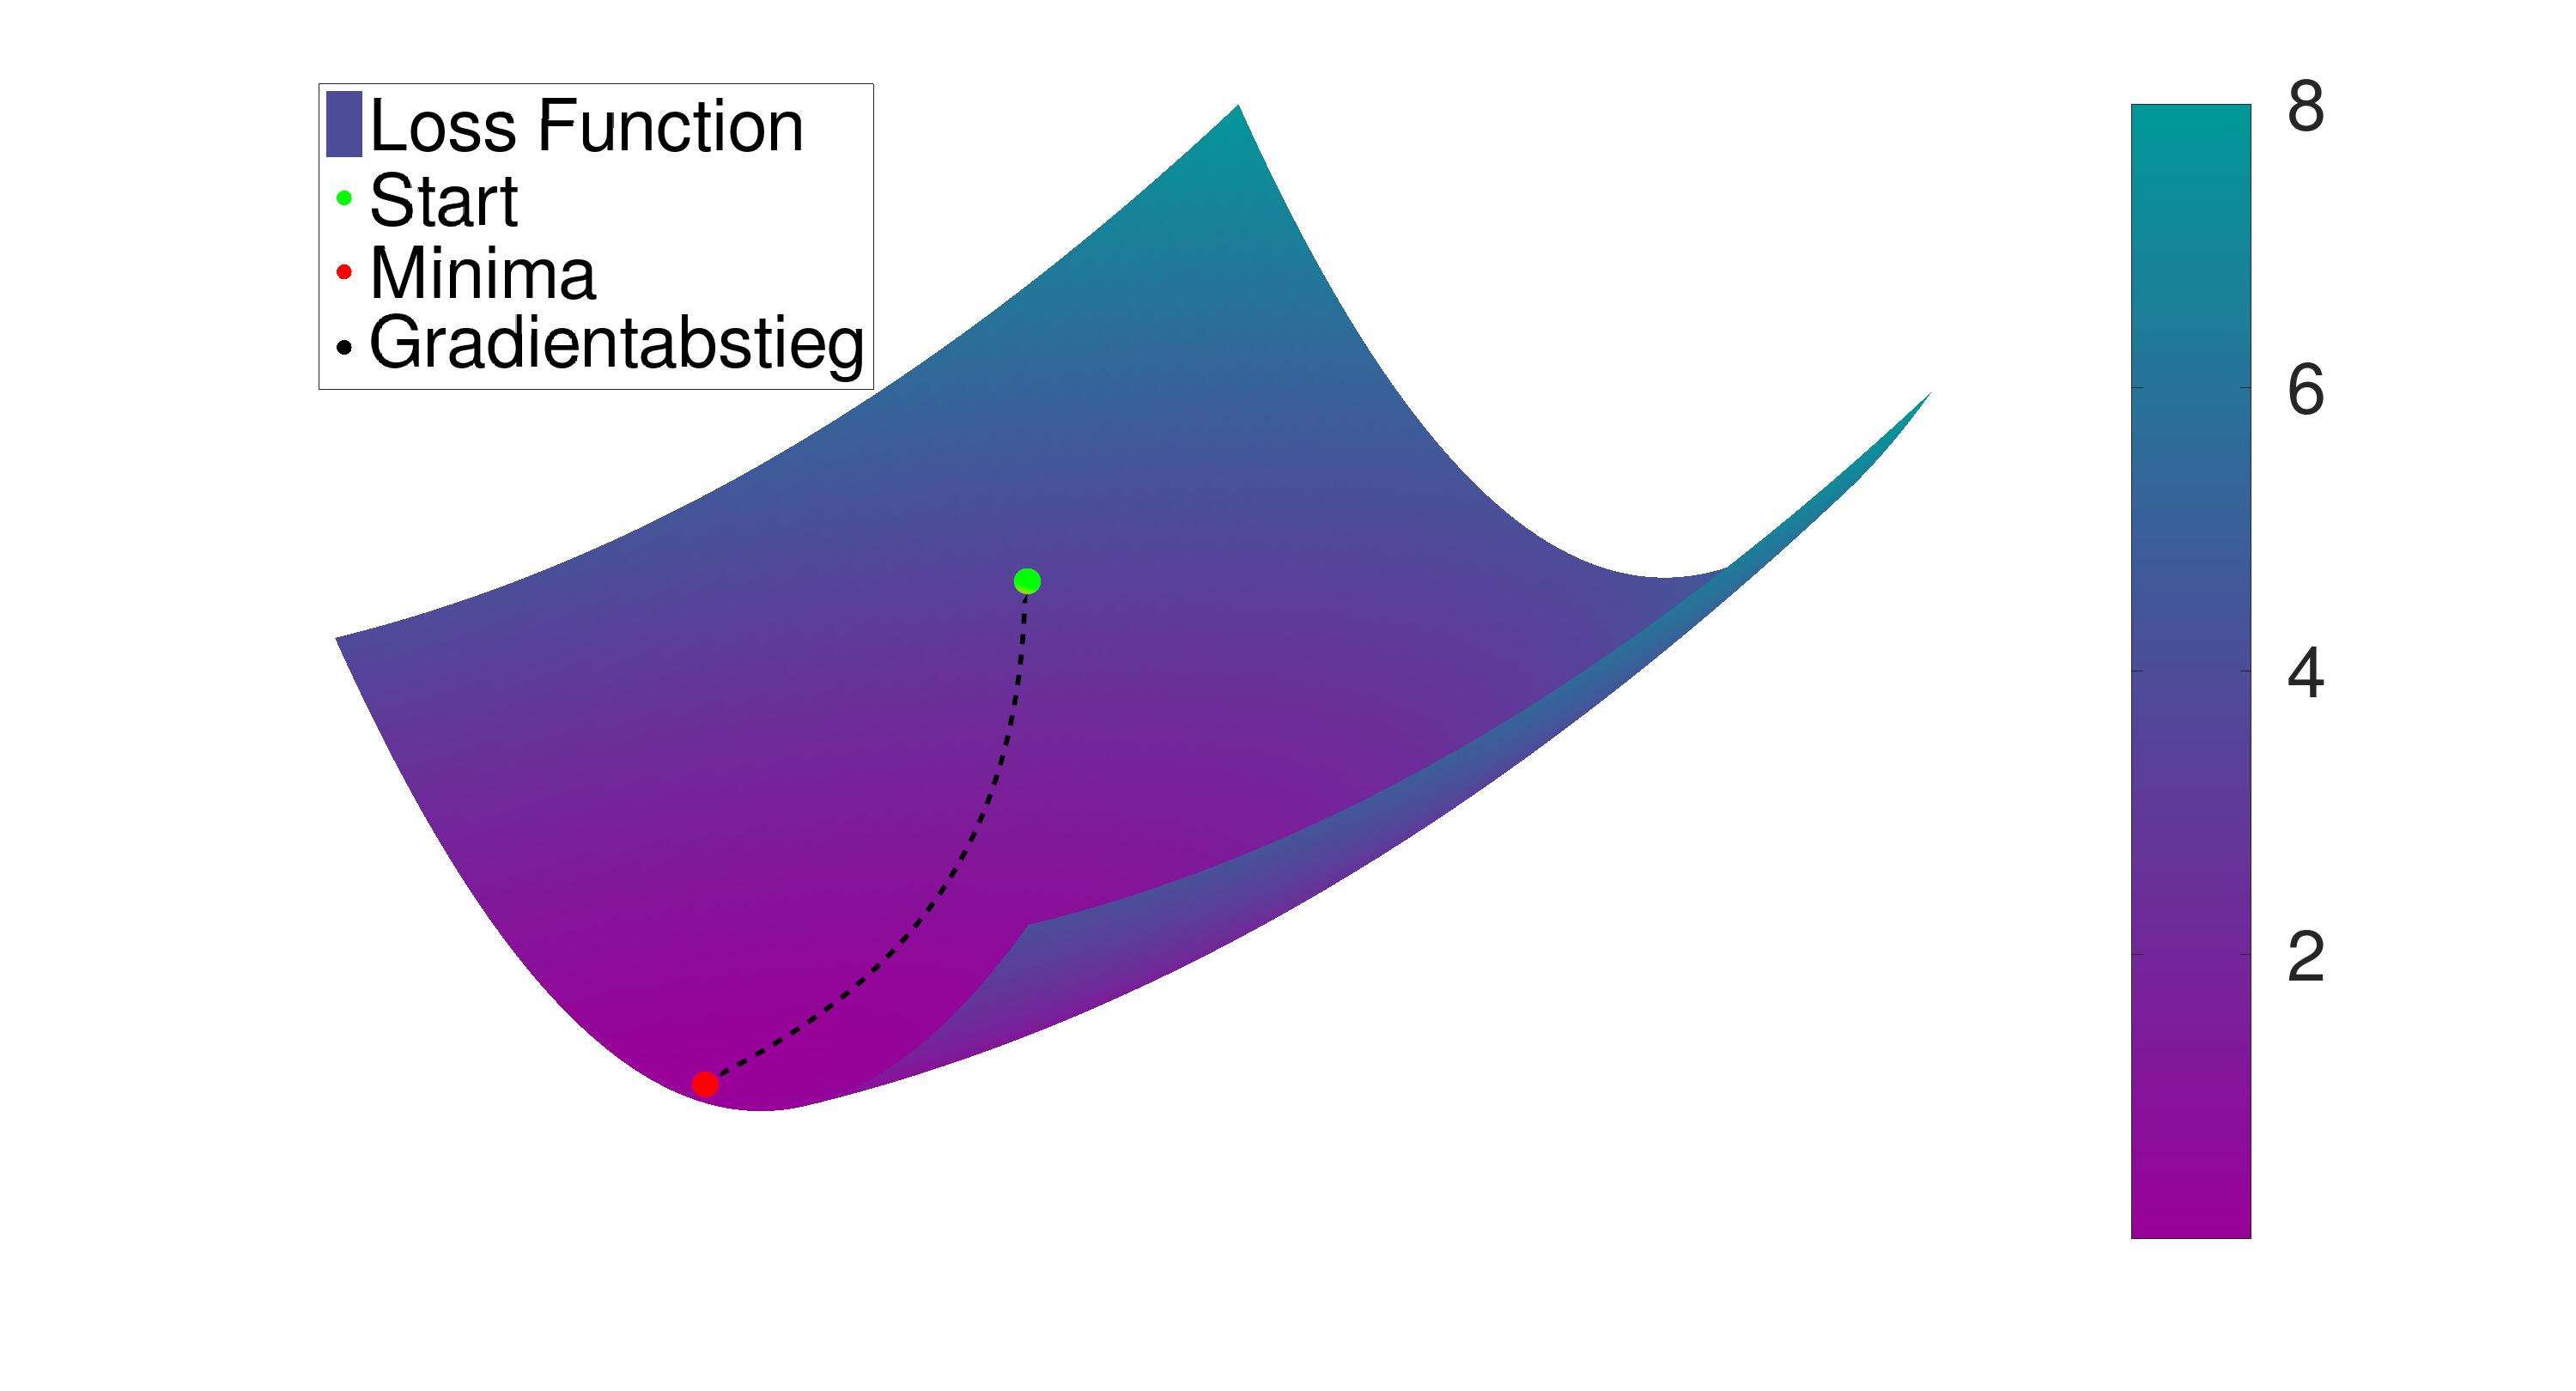
\includegraphics[width=0.9\textwidth]{papers/neuronal/images/gd_close_to_minima_long_distances_with_line.png}
    \caption{Beispiel eines Gradientenabstiegs zu einem lokalen Minimum}
    \label{fig:gradientenabstieg_beispiel}
\end{figure}


\subsubsection{Grenzen des Optimierungsverfahren}\label{neuronal:subsubsection:optimierungsverfahren_grenzen}

Der Algorithmus passt die Parameter des neuronalen Netzwerks schrittweise an, um die Funktion \( L(\vartheta) \) zu minimieren. 
Dieses Vorgehen birgt gewisse Risiken:
\begin{itemize}
    \item \textbf{Lokale Minima:} Der Algorithmus kann in einem lokalen Minimum stecken bleiben, insbesondere bei Funktionen mit vielen lokalen Minima.
\index{Minima, lokale}%
    \item \textbf{Sattelpunkte und Maxima:} Der Algorithmus kann auf Sattelpunkten oder Maxima landen, wo der Gradient ebenfalls null ist und keine weitere Bewegung möglich ist.
\index{Maxima}%
\index{Sattelpunkt}%
\end{itemize}

Lokale Minima sind nicht unbedingt ein Problem. 
Ist der Wert von $L$, bzw. der Approximationsfehler, an einem lokalen Minimum sehr tief, kann dies ausreichend zur Approximation sein.

Sattelpunkte und Maxima sind ein grösseres Problem, jedoch ist es unwahrscheinlich dass der Algorithmus einen solchen Punkt findet.
Grund dafür ist, dass der Algorithmus genau auf diesen Punkten landen müsste.
Ein bisschen daneben bedeutet dass es eine Richtung gibt, in die es abwärts --- und somit weg von diesen Punkten --- geht.

\subsection{Qualitätsbewertung}\label{neuronal:subsection:qualitätsbewertung}
\kopfrechts{Qualitätsbewertung}
\index{Qualitatsbewertung@Qualitätsbewertung}%
Für die Beurteilung der Qualität der Approximation bietet sich zunächst der Wert von \( L(\vartheta) \) nach Abschluss des Optimierungsalgorithmus an.
Dieser Wert entspricht dem mittleren Approximationsfehler, der bei den Datenpunkten aus der Diskretisierung auftritt.

Eine weitere Möglichkeit ist es, die drei Datensätze aus \ref{neuronal:subsection:diskretierung} in je zwei Teile aufzuteilen
\begin{equation*}
    \begin{aligned}
        F &= F_t \cup F_k\\
        A &= A_t \cup A_k\\
        B &= B_t \cup B_k.
    \end{aligned}
\end{equation*}
In der Funktion $L(\vartheta)$ wird über die drei Teil-Datensätze mit Index $t$ summiert.
Zudem wird eine neue Funktion \( L^1(\vartheta) \) analog zu $L(\vartheta)$ definiert, mit dem Unterschied, dass nun über die drei Teil-Datensätze mit Index $k$ summiert wird.
Da diese Funktion nie explizit durch den Optimierungsalgorithmus minimiert wurde, dient sie als Mass für den mittleren Approximationsfehler bei Datenpunkten, die nicht in der Diskretisierung enthalten waren.
Damit dies gilt, muss sichergestellt werden, dass $F_t \cap F_k = \emptyset$ ist (analog für $A$ und $B$), ansonsten ist $L^1(\vartheta)$ nicht unabhängig von $L(\vartheta)$.

Eine letzte Möglichkeit zur Qualitätsbewertung ist der direkte Vergleich mit Lösungen, die durch alternative Verfahren gefunden wurden.
Existiert beispielsweise eine analytische Lösung der Feldgleichung oder wurde eine Lösung durch die Finite-Element-Methode gefunden, kann damit verglichen werden.
\index{Finite-Element-Methode}%

%
% 2_beispiel.tex -- Wellengleichung tatsächlich lösen mit der Methode
%
% (c) 2025 Roman Cvijanovic & Nicola Dall'Acqua, Hochschule Rapperswil
%
% !TEX root = ../../buch.tex
% !TEX encoding = UTF-8
%

\section{Rechenbeispiele}\label{neuronal:section:rechenbeispiel}
\kopfrechts{Rechenbeispiele}

In diesem Abschnitt wird die zuvor vorgestellte Methode auf die Wellengleichung in zwei Dimensionen und die Burgers-Gleichung in einer Dimension angewendet.
Der Ablauf orientiert sich an den Schritten aus Abschnitt \ref{neuronal:section:herleitung}:
\begin{enumerate}
    \item Definition eines neuronalen Netzwerks
    \item Diskretisierung der Definitionsbereiche
    \item Aufbau der Funktion $L(\vartheta)$
    \item Minimierung von $L(\vartheta)$
    \item Qualitätsbewertung anhand von $L(\vartheta)$ und $L^1(\vartheta)$
\end{enumerate}

Sämtliche Resultate können mit dem Code im GitHub Repository \cite{neuronal:github_source_code} reproduziert werden.
Im Repository ist zusätzlich eine Readme-Datei abgelegt, welche einige Punkte bezüglich Reproduzierbarkeit klärt.

\subsection{Wellengleichung in zwei Dimensionen}\label{neuronal:subsection:wellengleichung}
Die zu lösende Gleichung lautet
\begin{equation}
    \frac{\partial^2 u}{\partial t^2} = c^2 \left( \frac{\partial^2 u}{\partial x^2} + \frac{\partial^2 u}{\partial y^2} \right).
    \label{neuronal:wellengleichung}
\end{equation}
Die Konstante \( c \) ist die Ausbreitungsgeschwindigkeit der Welle. Der Einfachheit halber wird \( c = 1 \) festgelegt.
Zusätzlich werden die folgenden Anfangsbedingungen
\begin{equation}
    \begin{aligned}
        u(x, y, 0) &= \sin(\pi x) \sin(\pi y)\\
        \frac{\partial u(x, y, 0)}{\partial t} &= 0
    \end{aligned}
    \label{neuronal:wellen_anfangs}
\end{equation}
sowie die Randbedingungen
\begin{equation}
    \begin{aligned}
        u(-2, y, t) &= 0\\
        u(2, y, t) &= 0\\
        u(x, -2, t) &= 0\\
        u(x, 2, t) &= 0
    \end{aligned}
    \label{neuronal:wellen_rand}
\end{equation}
verwendet.
Die Bereiche sind \( x, y \in [-2,2] \) und \( t \in [0,2] \).
Dieses Gleichungssystem hat eine analytische Lösung welche
\begin{equation}
    u(x, y, t) = \cos(c \pi \sqrt{2}\: t)\sin(\pi x)\sin(\pi y)
    \label{neuronal:wellen_analytisch}
\end{equation}
lautet.
Somit kann das neuronale Netzwerk zur Qualitätsbewertung direkt damit verglichen werden.

Das neuronale Netzwerk zur Lösung der Wellengleichung weicht leicht von der allgemeinen Definition im Abschnitt \ref{neuronal:subsection:struktur_nn} ab.
Zusätzlich zu den drei Variablen $x, y$ und $t$ wird dem Netzwerk der Wert der ersten Anfangsbedingung \eqref{neuronal:wellen_anfangs} als Input gegeben.
Somit ist das neuronale Netzwerk
\begin{align*}
    \hat{u}(x,\; y,\; t,\; u(x, y, 0);\; \vartheta),
\end{align*}
wobei
\begin{align*}
    u(x, y, 0) = \sin(\pi x) \sin(\pi y).
\end{align*}
Die Idee dabei ist, dass diese Anfangsbedingung auf eine bestimmte Art in der gesuchten Funktion $u$ vorkommen muss.
Daher ist es naheliegend, diese Anfangsbedingung als zusätzlichen Input zu verwenden.
Der konkrete Aufbau des neuronalen Netzwerks ist somit wie folgt:
\begin{itemize}
    \item 4 Teilfunktionen
    \item \( f_1 \): \( \mathbb{R}^4 \longrightarrow \mathbb{R}^{128} \) 
    \item \( f_{4} \): \( \mathbb{R}^{128} \longrightarrow \mathbb{R} \)
    \item Alle anderen Teilfunktionen: \( \mathbb{R}^{128} \longrightarrow \mathbb{R}^{128} \)
    \item Als Aktivierungsfunktion wird der hyperbolische Tangens verwendet
\end{itemize}
Das Netzwerk verfügt somit über 33'793 Parameter.
In der letzten Teilfunktion \( f_{4} \) wird keine Aktivierungsfunktion verwendet.
Grund dafür ist, dass der hyperbolische Tangens den Wertebereich \((-1, 1)\) hat, das Netzwerk aber zur Approximation der Wellengleichung den Wertebereich \( \mathbb{R} \) haben soll.

Wie im Abschnitt \ref{neuronal:subsection:diskretierung} beschrieben, werden insgesamt drei Datensätze verwendet.
Alle drei Datensätze bestehen aus je 50'000 Datenpunkten.
Weiter wurde je ein Fünftel der Datenpunkte für die Funktion \( L^1(\vartheta) \) abgetrennt und nicht im Optimierungsalgorithmus verwendet (siehe Abschnitt \ref{neuronal:subsection:qualitätsbewertung}).

Beendet man den Optimierungsalgorithmus nach 1500 Iterationen, findet sich eine gute Lösung.
Die Werte von $L(\vartheta)$ und $L^1(\vartheta)$ sind 4.011 bzw. 0.878 (siehe Abbildung \ref{fig:fehler_wave_good}), was zunächst nicht besonders vielversprechend ist.
Zusätzliche Iterationen des Optimierungsalgorithmus reduzieren zwar den Wert von $L(\vartheta)$ weiter, doch der Wert von $L^1(\vartheta)$ beginnt wieder anzusteigen.
Dies ist ein klassisches Phänomen im Gebiet des maschinellen Lernens und wird als \emph{Overfitting} bezeichnet.
\emph{Overfitting} bedeutet, dass das neuronale Netzwerk die Datenpunkte $F_t\cup A_t \cup B_t$, mit denen $L(\vartheta)$ berechnet wird, ``auswendig'' lernt.
Als Resultat versagt das Netzwerk bei den Datenpunkten $F_k\cup A_k \cup B_k$, mit denen $L^1(\vartheta)$ berechnet wird.
Daher wurde der Optimierungsalgorithmus nach 1500 Iterationen beendet, obwohl die Approximationsfehler nicht sehr tief sind.
\begin{figure}
    \centering
    \hspace*{-0.1\textwidth}
    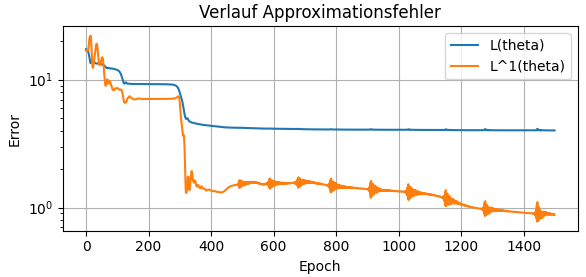
\includegraphics[width=0.7\textwidth]{papers/neuronal/images/approximation_error_wave_good.png}
    \caption{Verlauf des Approximationsfehlers der Wellengleichung während des Trainings}
    \label{fig:fehler_wave_good}
\end{figure}

Berechnet man nun die durchschnittliche Differenz des neuronalen Netzwerks und der analytischen Lösung \eqref{neuronal:wellen_analytisch}, erhält man 0.079.
Dieser Wert ist deutlich besser und deutet darauf hin, dass das neuronale Netzwerk eine gute Approximation liefert. 
Der Verlauf dieser Differenz ist in \ref{fig:differenz_wellen} dargestellt.
\begin{figure}
    \centering
    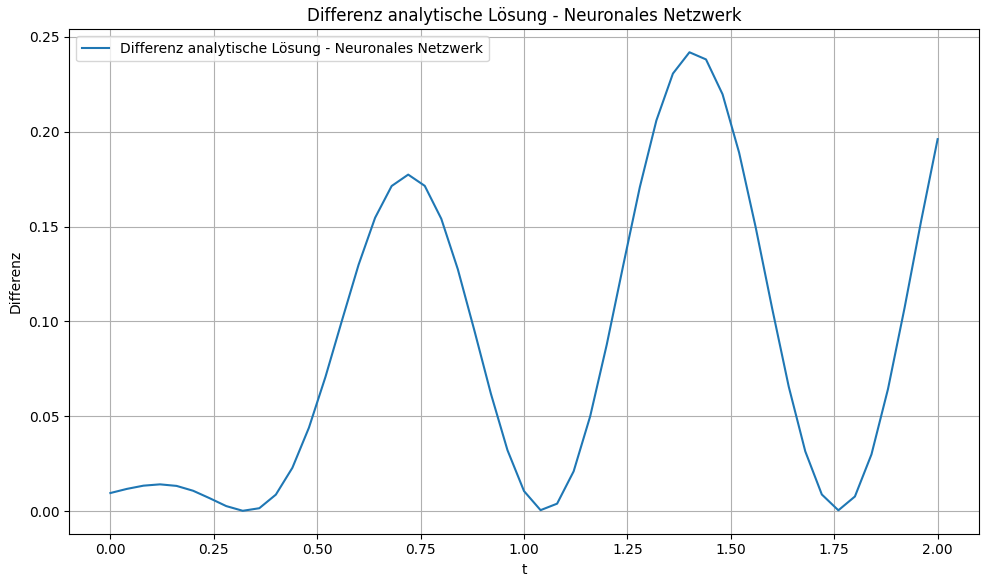
\includegraphics[width=0.7\textwidth]{papers/neuronal/images/wellen_analytisch_neuronal.png}
    \caption{Verlauf der Differenz Wellengleichung: Analytische Lösung - Neuronales Netzwerk}
    \label{fig:differenz_wellen}
\end{figure}

Der Lösungsplot ist in den Abbildungen \ref{fig:wellen_t0}, \ref{fig:wellen_t04}, \ref{fig:wellen_t136}, \ref{fig:wellen_t164} dargestellt.
In diesen Abbildungen ist auf der linken Seite das neuronale Netzwerk und auf der rechten Seite die analytische Lösung abgebildet.
Die Farben stellen die Wellenhöhen dar, rot bedeutet einen Wellenberg und blau ein Wellental.
Was in diesen Abbildungen deutlich zu sehen ist, ist dass das Netzwerk bei Übergängen von Wellenbergen zu Wellentälern (z.B. von \ref{fig:wellen_t0} zu \ref{fig:wellen_t04}) Fehler macht.
Dies wird deutlich wenn man $y$ bei $0.5$ fixiert und Lösungsplots für verschiedene $t$ erstellt (siehe Abbildung \ref{fig:loesung_wellen_fix_yt}).
In dieser Abbildungsreihe ist klar zu erkennen, dass diese Übergänge zwar stattfinden, aber chaotisch ablaufen.
Abgesehen davon sieht die Approximation visuell gut aus.
Die Approximation ist als Animation über den gesamten Zeitraum $t \in [0, 2]$ im GitHub Repository des Seminars \cite{neuronal:github_source_code}, im Unterverzeichnis \emph{wave\_equation} zu finden.
\begin{figure}
    \centering
    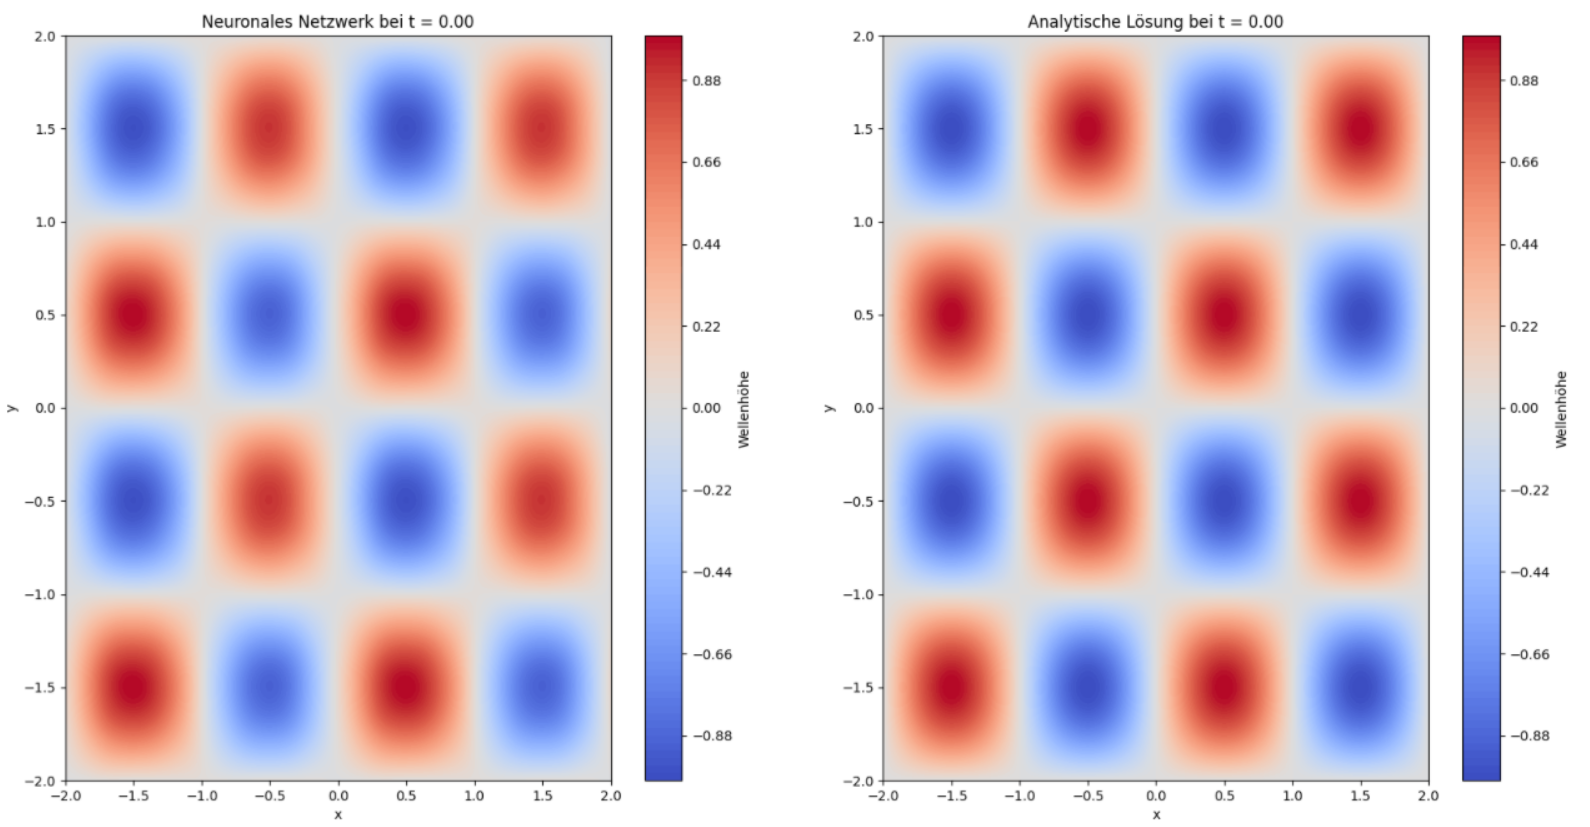
\includegraphics[width=\textwidth]{papers/neuronal/images/prediction_wave_t0.png}
    \caption{Wellengleichung t = 0}
    \label{fig:wellen_t0}
\end{figure}
\begin{figure}
    \centering
    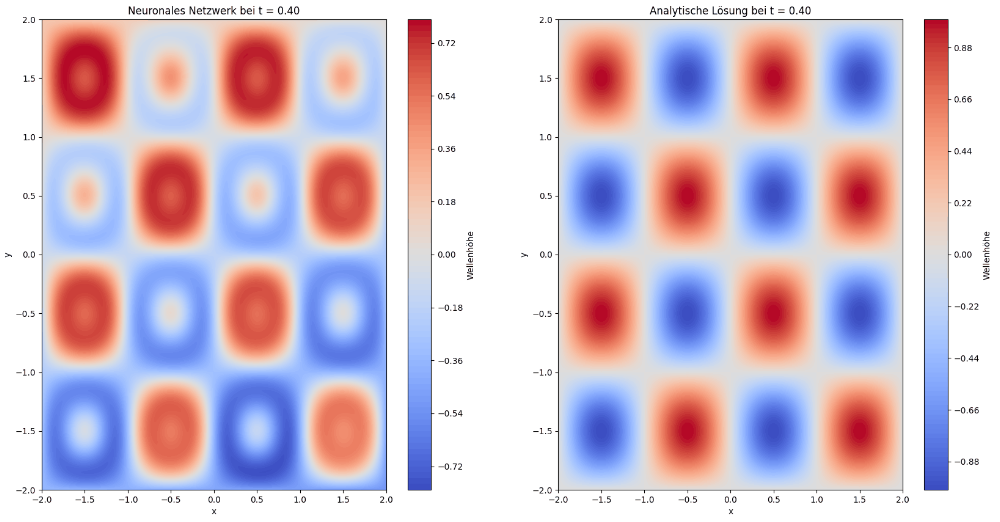
\includegraphics[width=\textwidth]{papers/neuronal/images/prediction_wave_t04.png}
    \caption{Wellengleichung t = 0.4}
    \label{fig:wellen_t04}
\end{figure}
\begin{figure}
    \centering
    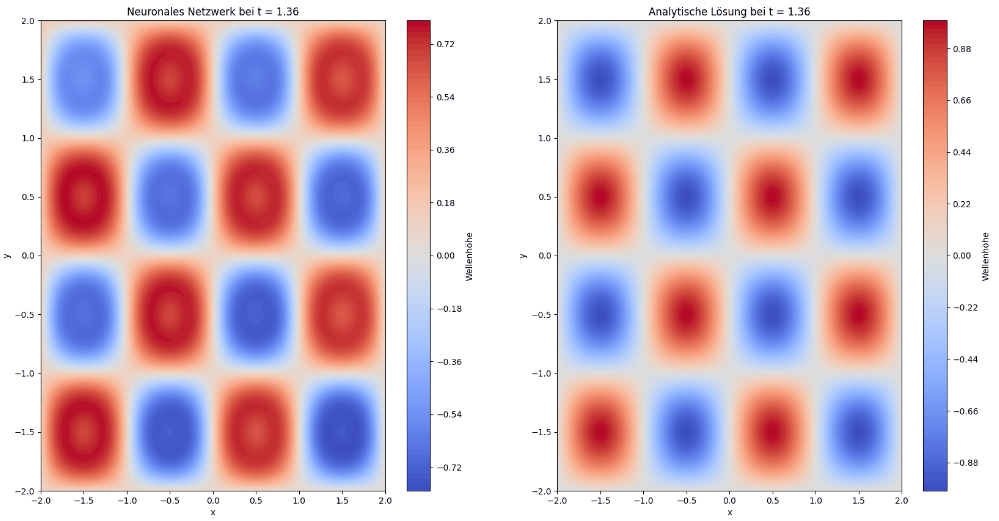
\includegraphics[width=\textwidth]{papers/neuronal/images/prediction_wave_t136.png}
    \caption{Wellengleichung t = 1.36}
    \label{fig:wellen_t136}
\end{figure}
\begin{figure}
    \centering
    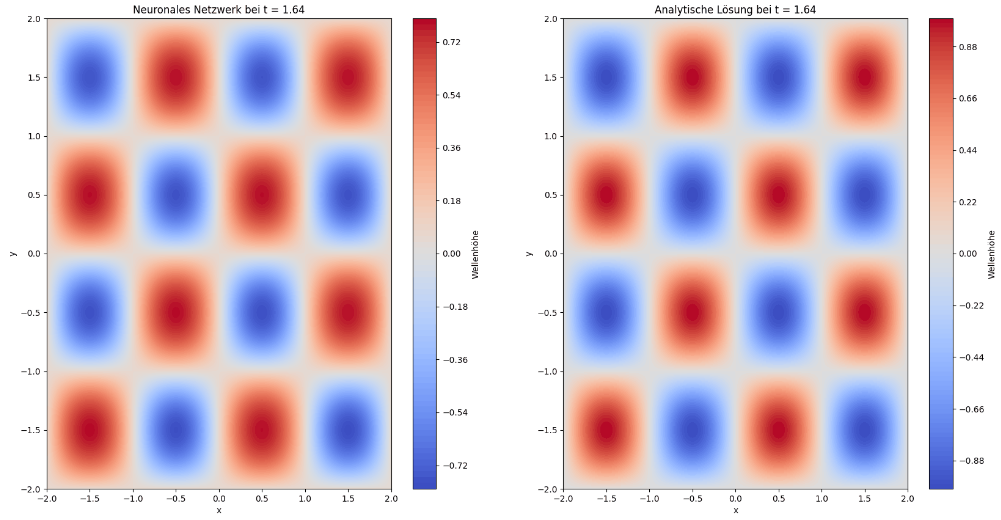
\includegraphics[width=\textwidth]{papers/neuronal/images/prediction_wave_t164.png}
    \caption{Wellengleichung t = 1.64}
    \label{fig:wellen_t164}
\end{figure}

\begin{figure}
    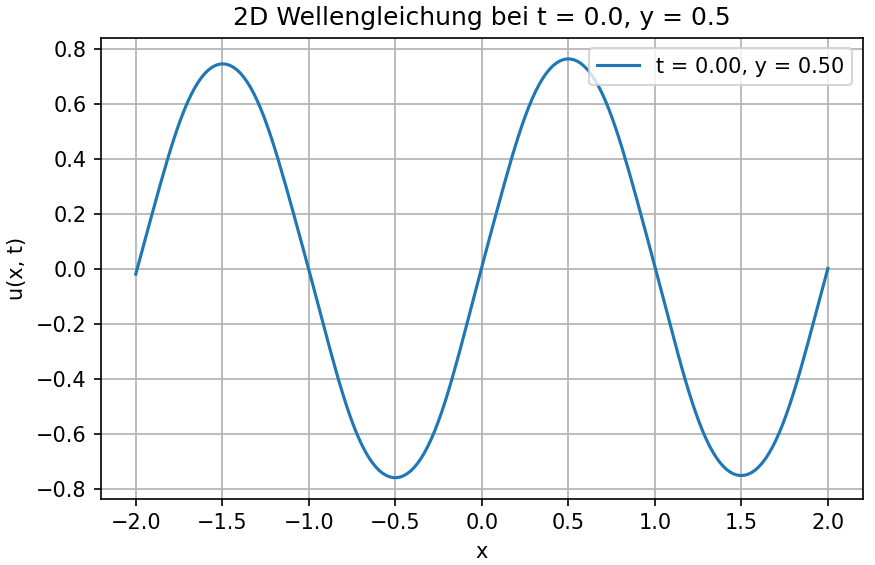
\includegraphics[width=0.48\textwidth]{papers/neuronal/images/wave_solution_t0.png}\hfill
    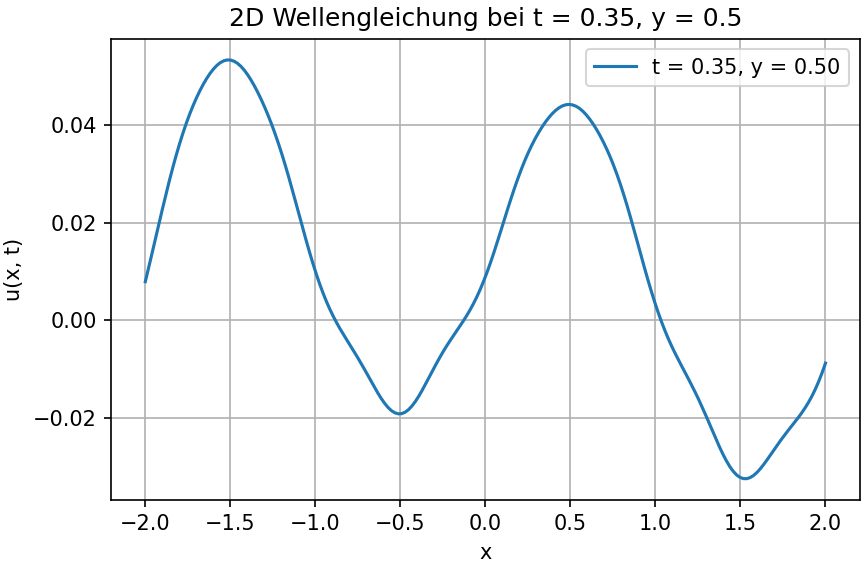
\includegraphics[width=0.48\textwidth]{papers/neuronal/images/wave_solution_t035.png}
    \\[\smallskipamount]
    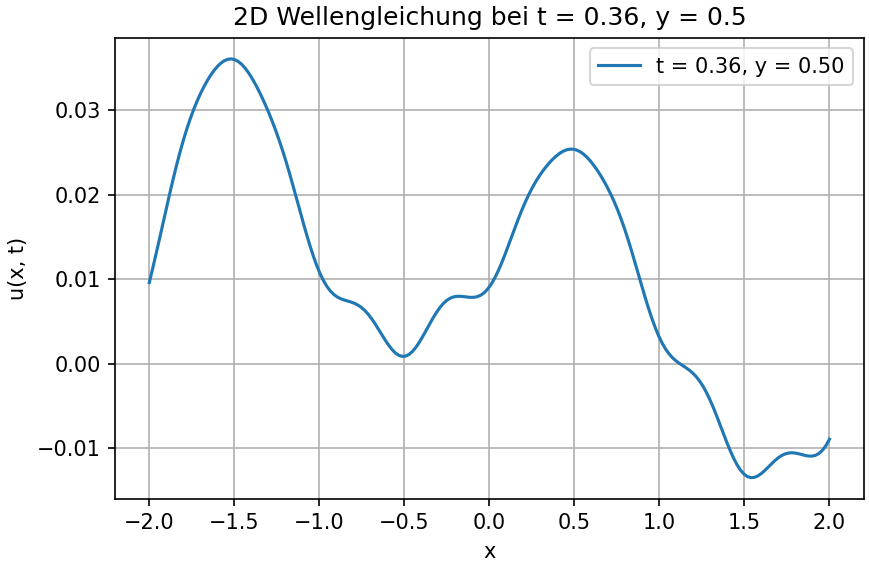
\includegraphics[width=0.48\textwidth]{papers/neuronal/images/wave_solution_t036.png}\hfill
    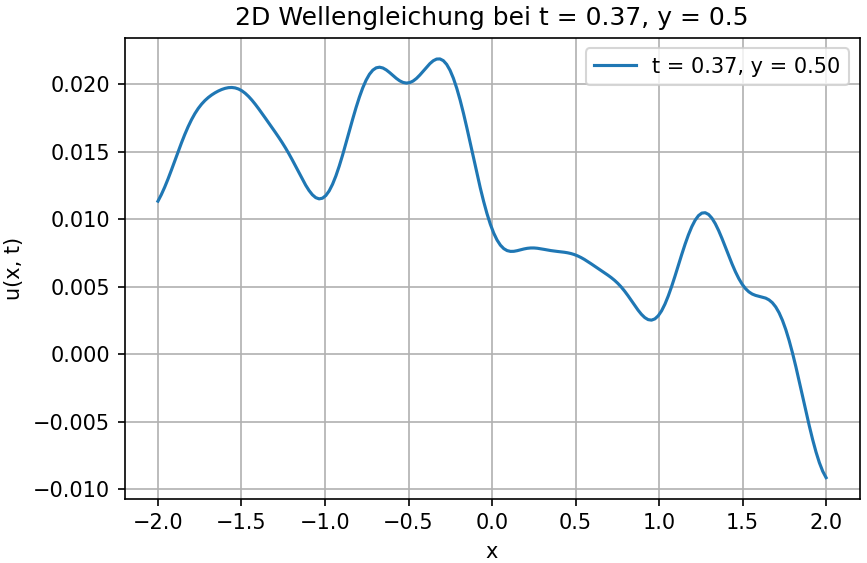
\includegraphics[width=0.48\textwidth]{papers/neuronal/images/wave_solution_t037.png}
    \\[\smallskipamount]
    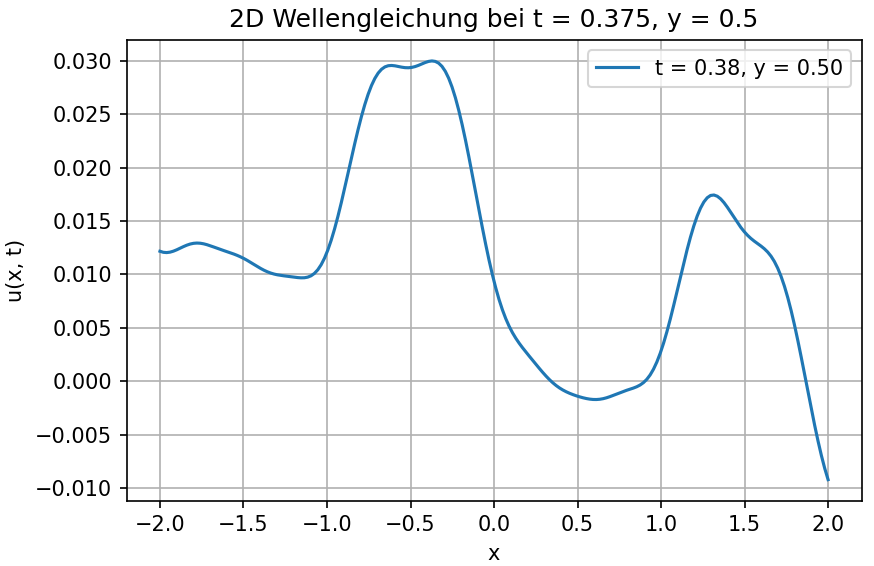
\includegraphics[width=0.48\textwidth]{papers/neuronal/images/wave_solution_t0375.png}\hfill
    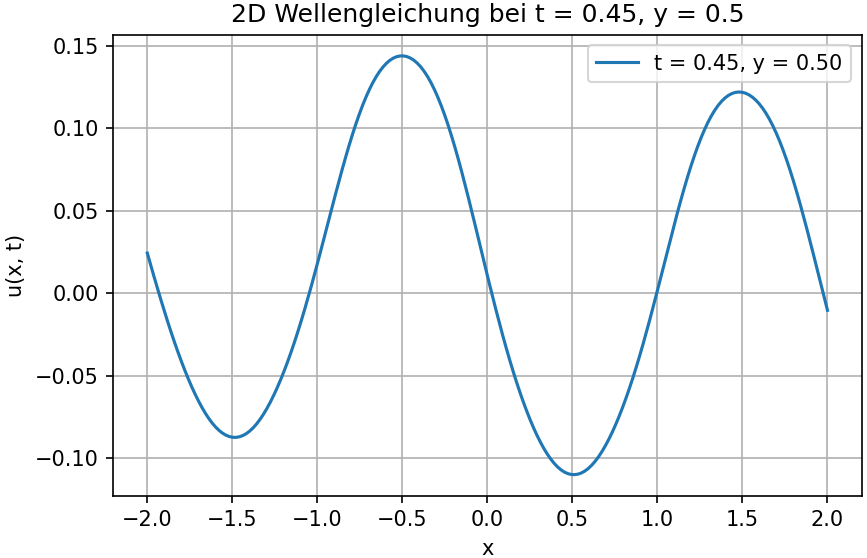
\includegraphics[width=0.48\textwidth]{papers/neuronal/images/wave_solution_t045.png}
    \caption{Lösungs-Plot der Wellengleichung zu verschiedenen Zeiten und y = 0.5}\label{fig:loesung_wellen_fix_yt}
\end{figure}

\subsection{Burgers-Gleichung}\label{neuronal:subsection:burgers_gleichung}
Die Burgers-Gleichung ist gegeben als
\begin{equation}
    \frac{\partial u}{\partial t} + u \frac{\partial u}{\partial x} = \nu \frac{\partial^2 u}{\partial x^2}.
    \label{neuronal:burgers}
\end{equation}
Der Diffusionskoeffizient \( \nu \) wird auf \( \nu = \frac{0.01}{\pi} \) festgelegt.
Die Anfangsbedingung
\begin{equation}
    u(0, x) = - \sin(\pi x)
    \label{neuronal:burgers_anfang}
\end{equation}
und die Randbedingung
\begin{equation}
    u(t, -1) = u(t, 1) = 0.
    \label{neuronal:burgers_rand}
\end{equation}
werden verwendet.
Die Bereiche sind \( x \in [-1,1] \) und \( t \in [0,1] \).

Das neuronale Netzwerk zur Lösung der Burgers-Gleichung ist folgendermassen aufgebaut:
\begin{itemize}
    \item 10 Teilfunktionen
    \item \( f_1 \): \( \mathbb{R}^2 \longrightarrow \mathbb{R}^{20} \) 
    \item \( f_{10} \): \( \mathbb{R}^{20} \longrightarrow \mathbb{R} \)
    \item Alle anderen Teilfunktionen: \( \mathbb{R}^{20} \longrightarrow \mathbb{R}^{20} \)
    \item Als Aktivierungsfunktion wird der hyperbolische Tangens verwendet
\end{itemize}
Das Netzwerk verfügt somit über 3441 Parameter.
In der letzten Teilfunktion \( f_{10} \) wird keine Aktivierungsfunktion verwendet.
Grund dafür ist, dass der hyperbolische Tangens den Wertebereich \((-1, 1)\) hat, das Netzwerk aber zur Approximation der Burgers-Gleichung den Wertebereich \( \mathbb{R} \) haben soll.

Wie im Abschnitt \ref{neuronal:subsection:diskretierung} beschrieben, werden insgesamt drei Datensätze verwendet.
Der Datensatz \( F \), in dem die Burgers-Gleichung gilt, besteht aus 5000 Datenpunkten.
Die Datensätze \( A \) und \( B \), in denen die Anfangsbedingungen bzw. die Randbedingungen gilten, bestehen jeweils aus 2000 Datenpunkten.
Weiter wurde je ein Fünftel der Datenpunkte für die Funktion \( L^1(\vartheta) \) abgetrennt und nicht im Optimierungsalgorithmus verwendet (siehe Abschnitt \ref{neuronal:subsection:qualitätsbewertung}).

Der Optimierungsalgorithmus \ref{neuronal:gradient_descent} durchlief 15'000 Iterationen, um geeignete Parameter für die Approximation zu finden.
Die Werte von \( L(\vartheta) \) und \( L^1(\vartheta) \) am Ende der Optimierung sind 0.003328 bzw. 0.003449.
Somit sind die mittleren Approximationsfehler des Netzwerks sehr gering.
Der Verlauf des Approximationsfehlers während der Optimierung ist in Abbildung \ref{fig:fehler_burgers} dargestellt.
\begin{figure}
    \centering
    \hspace*{-0.1\textwidth}
    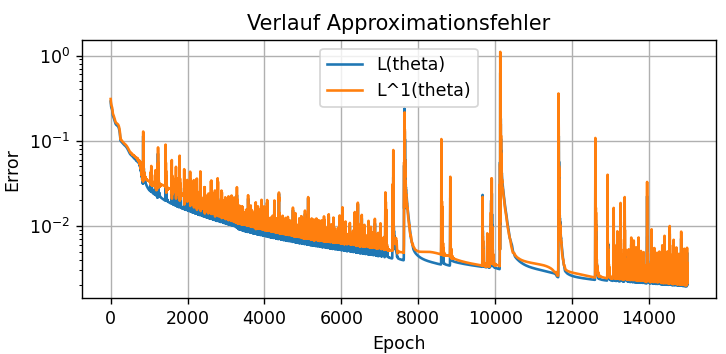
\includegraphics[width=0.7\textwidth]{papers/neuronal/images/approximation_error_burgers.png}
    \caption{Verlauf des Approximationsfehlers der Burgers-Gleichung während des Trainings}
    \label{fig:fehler_burgers}
\end{figure}

Wertet man das neuronale Netzwerk über die Bereiche von \( x \) und \( t \) aus, ergibt sich ein Plot der Lösung des neuronalen Netzwerks (siehe Abbildung \ref{fig:loesung_burgers}).
In dieser Abbildung laufen zwei sanfte Wellen aufeinander zu und kollidieren in einem scharfen Sprung.
\begin{figure}
    \centering
    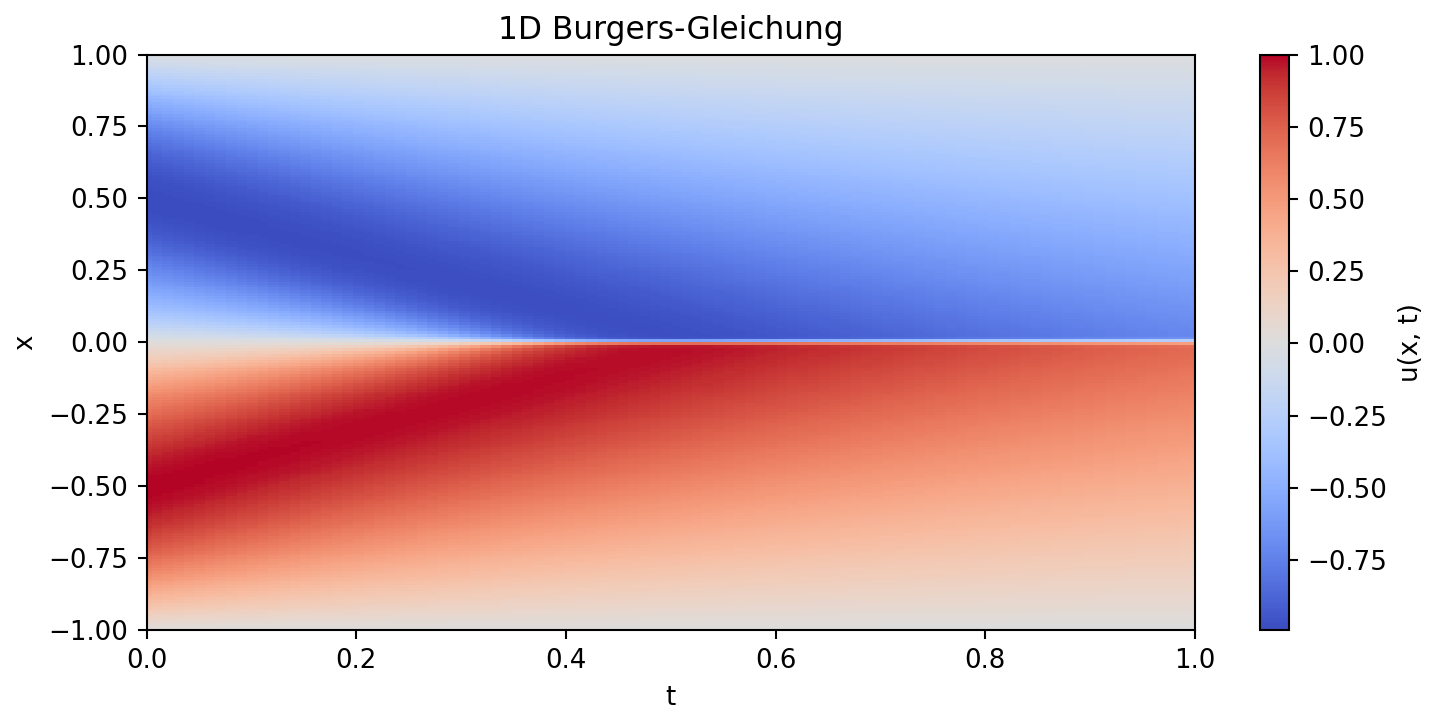
\includegraphics[width=0.8\textwidth]{papers/neuronal/images/prediction_burgers_net.png}
    \caption{Lösungs-Plot der Burgers-Gleichung}
    \label{fig:loesung_burgers}
\end{figure}
Dieses Verhalten wird deutlich, wenn man den Lösungsplot zu fixen Zeiten erstellt, siehe \ref{fig:loesung_burgers_fix_zeit}.
\begin{figure}
    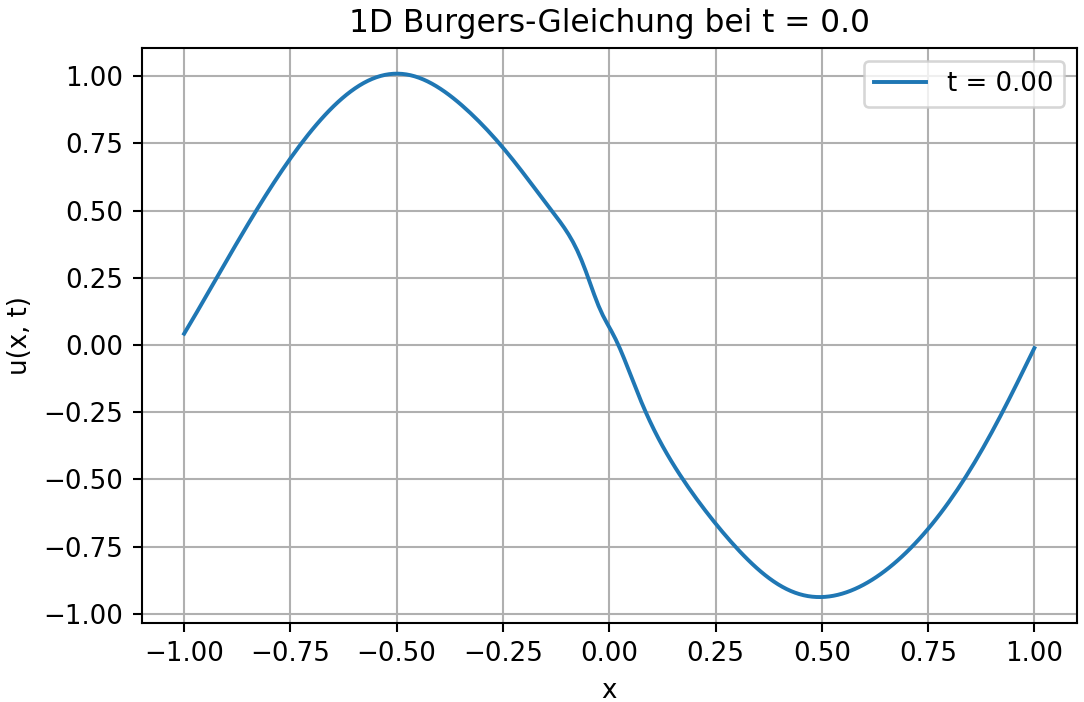
\includegraphics[width=0.48\textwidth]{papers/neuronal/images/burgers_solution_t0.png}\hfill
    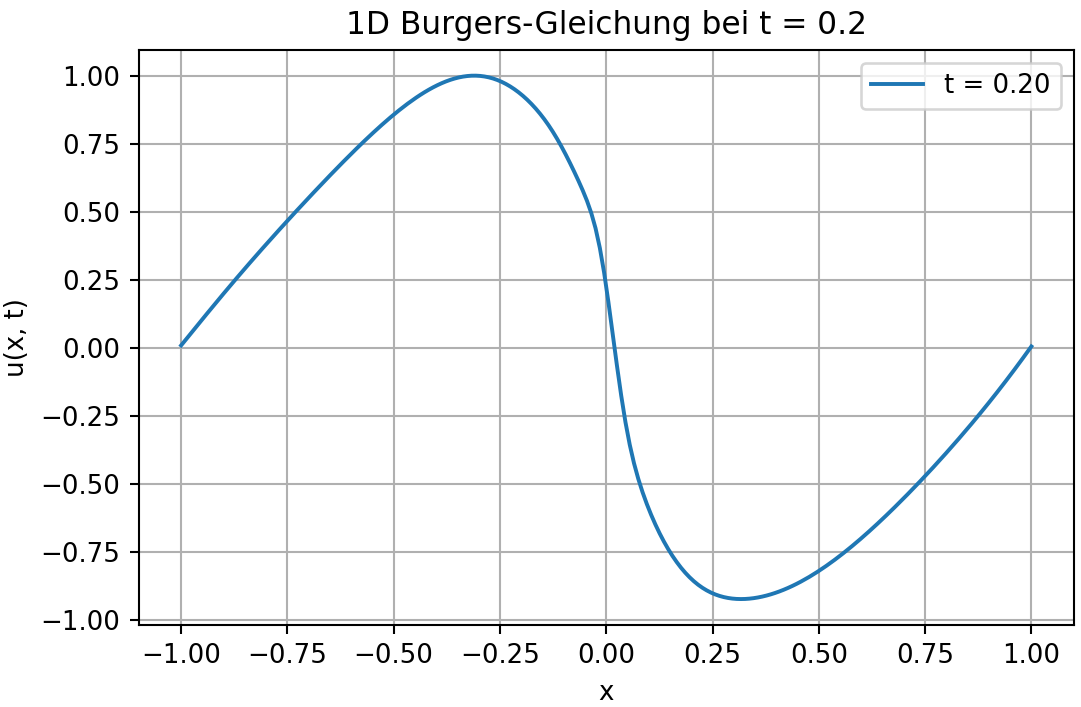
\includegraphics[width=0.48\textwidth]{papers/neuronal/images/burgers_solution_t02.png}
    \\[\smallskipamount]
    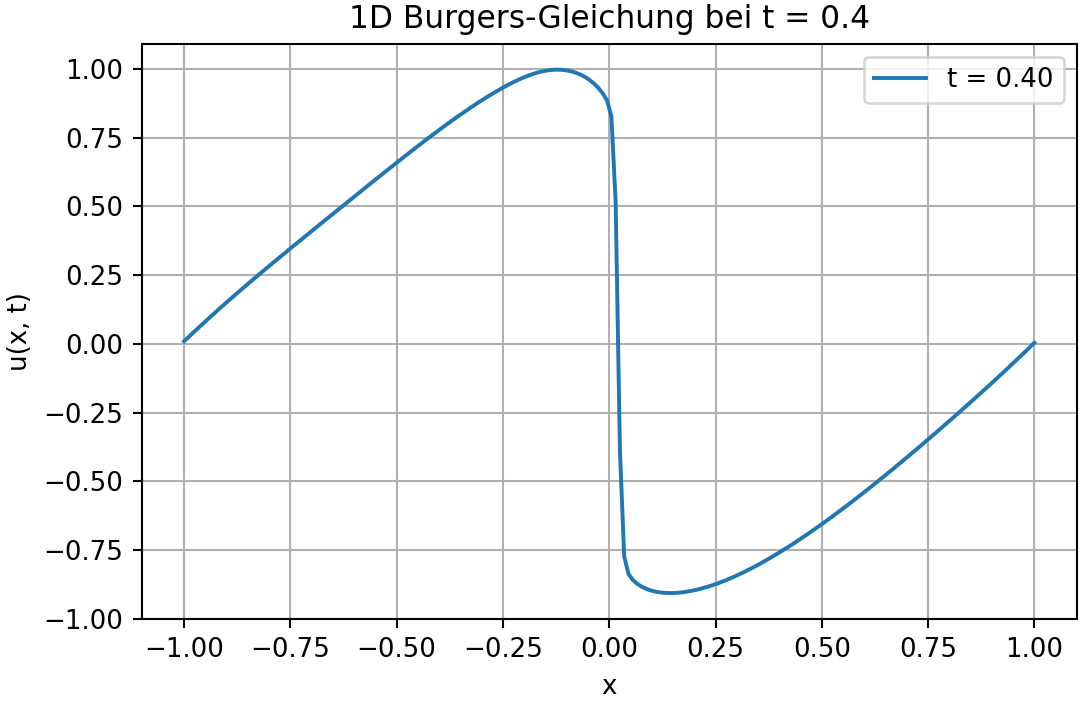
\includegraphics[width=0.48\textwidth]{papers/neuronal/images/burgers_solution_t04.png}\hfill
    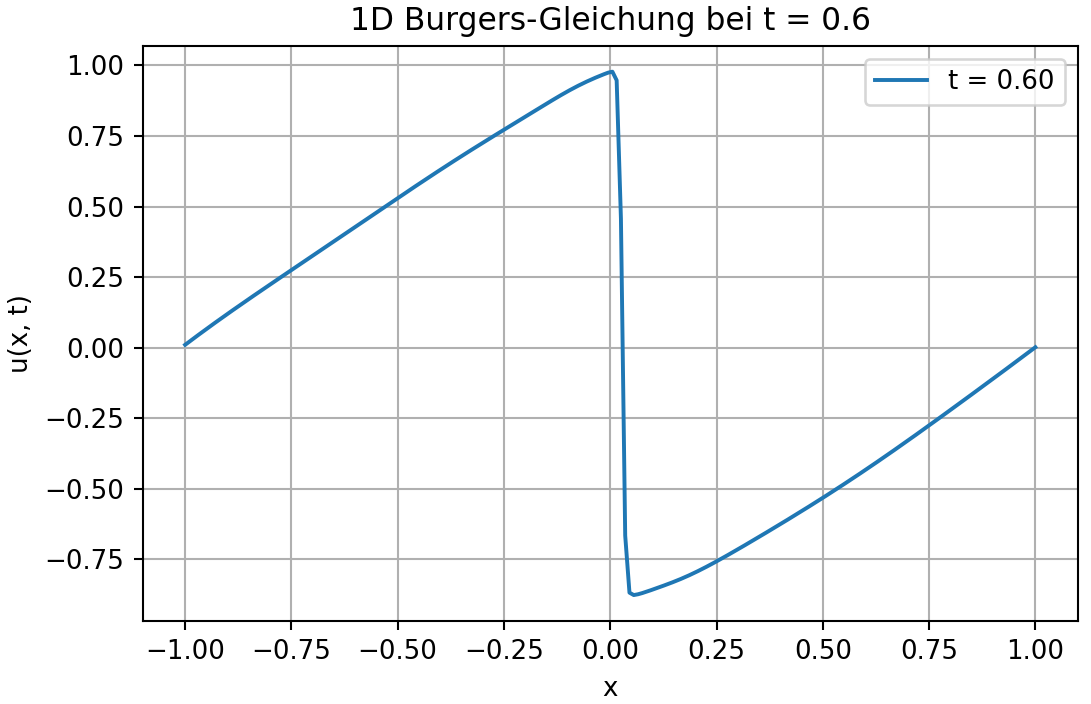
\includegraphics[width=0.48\textwidth]{papers/neuronal/images/burgers_solution_t06.png}
    \caption{Lösungs-Plot der Burgers-Gleichung zu verschiedenen Zeiten}\label{fig:loesung_burgers_fix_zeit}
\end{figure}

Der gesamte Code zur Umsetzung ist im GitHub-Repository des Seminars abgelegt \cite{neuronal:github_source_code}.


%
% 3_weiteres.tex -- Diskussion & weitere Anwendungsmöglichkeiten
%
% (c) 2025 Roman Cvijanovic & Nicola Dall'Acqua, Hochschule Rapperswil
%
% !TEX root = ../../buch.tex
% !TEX encoding = UTF-8
%

\section{Diskussion}\label{neuronal:section:diskussion}
\kopfrechts{Diskussion}

Der grosse Vorteil dieser Methode liegt in ihrer breiten Anwendbarkeit.
Sie kann grundsätzlich auf beliebige Feldgleichungen angewendet werden, unabhängig von deren Komplexität.
Im Gegensatz dazu sind klassische Verfahren wie die Finite-Differenzen- oder Finite-Elemente-Methode oft auf bestimmte Gleichungstypen beschränkt und stossen insbesondere bei stark nichtlinearen oder hochdimensionalen Problemen an ihre Grenzen.
\index{Finite-Differenzen-Methode}%
\index{Finite-Element-Methode}%
Neuronale Netzwerke bieten durch das \emph{Universal Approximation Theorem} die theoretische Grundlage, um beliebige stetige Funktionen mit beliebiger Genauigkeit zu approximieren \cite{neuronal:universal_approximation_theorem}.
\index{Universal Approximation Theorem}%
Dies befähigt sie theoretisch dazu, Lösungen für jede beliebige Feldgleichung zu approximieren.

Was die vorangegangenen Beispiele jedoch klar zeigen, ist dass diese Methode bei der Burgers-Gleichung deutlich besser funktioniert als bei der Wellengleichung.
Der Grund dafür liegt in den Gleichungen selbst: 
Die Wellengleichung ist eine hyperbolische, die Burgers-Gleichung eine parabolische partielle Differentialgleichung.
\index{partielle Differentialgleichung!hyperbolische}%
\index{hyperbolisch}%
\index{partielle Differentialgleichung!parabolische}%
\index{parabolisch}%
Neuronale Netzwerke haben beim Lösen von hyperbolischen Gleichungen Schwierigkeiten \cite{neuronal:hyperbolisch_1}, \cite{neuronal:hyperbolisch_2}, \cite{neuronal:hyperbolisch_3}.
Zu beachten ist, dass diese Schwierigkeiten nicht auf einen Mangel an Ausdruckskraft des neuronalen Netzwerks zurückzuführen sind.
Vielmehr liegt der Grund im Lösen des vorgestellten Optimierungsproblems \ref{neuronal:subsection:lösen_optimierungsproblem} \cite{neuronal:hyperbolisch_4}.
Dieses wird für bestimmte Gleichungstypen, wie hyperbolische Feldgleichungen, durch deren charakteristische Eigenschaften --- zum Beispiel kontinuierliche Wellenausbreitung --- erheblich erschwert.
Dadurch kann das Finden einer guten Lösung sehr schwer werden.
Somit ist die Existenz einer guten Lösung zwar durch das \emph{Universal Approximation Theorem} garantiert, nicht aber das Finden davon.

In der Praxis zeigen neuronale Netzwerke vielversprechende Ergebnisse beim Lösen von Feldgleichungen \cite{neuronal:pinns}.
Jedoch befindet sich die Methode noch in einem frühen Entwicklungsstadium.
Es gibt viele offene Fragen, insbesondere hinsichtlich der Effizienz und Genauigkeit im Vergleich zu klassischen Verfahren.
Zusätzliche Forschungsergebnisse dürften hierzu weitere Erkenntnisse liefern.
Eine abschließende Bewertung der Methode ist daher zum jetzigen Zeitpunkt noch nicht möglich.


\printbibliography[heading=subbibliography]
\end{refsection}
